\PassOptionsToPackage{dvipsnames}{xcolor}
\documentclass[border=3mm]{standalone}
\usepackage[dvipsnames]{xcolor}
\usepackage{amsmath}
\usepackage{amssymb}
\usepackage{dsfont}
\usepackage{bm}
\usepackage{tikz}
\usetikzlibrary{arrows}
\usetikzlibrary{calc}



\definecolor{color1}{rgb}{0,0.4470,0.7410}
\definecolor{color2}{rgb}{0.8500,0.3250,0.0980}
\definecolor{color3}{rgb}{0.9290,0.6940,0.1250}
\definecolor{color4}{rgb}{0.4940,0.1840,0.5560}
\definecolor{color5}{rgb}{0.4660,0.6740,0.1880}


\begin{document}



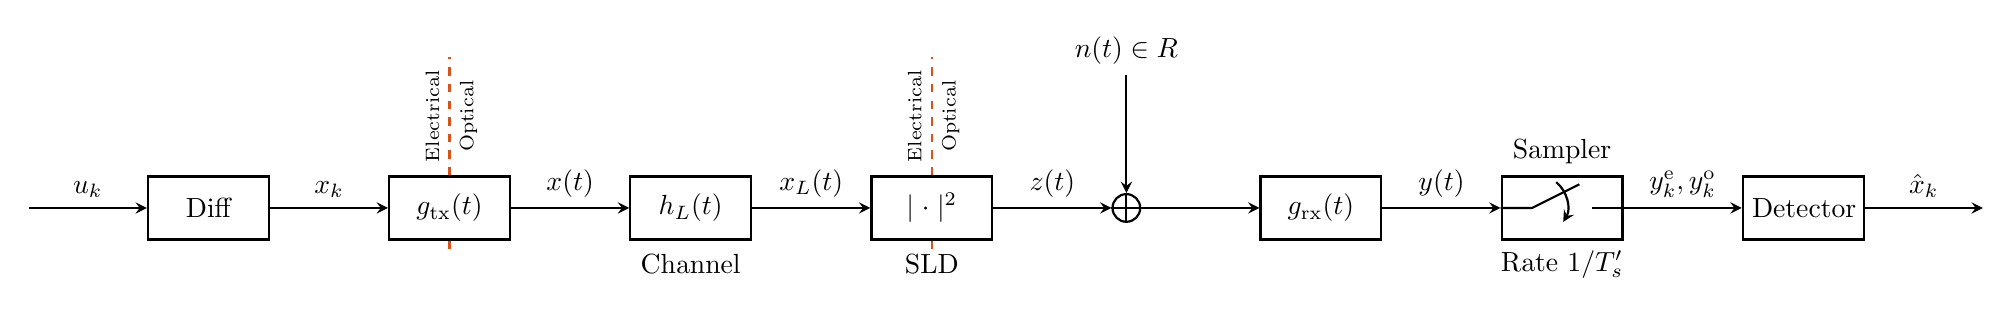
\begin{tikzpicture}[>=stealth,thick]

\node [rectangle, draw, text width = 1.3cm, minimum height = 0.8cm, align = center, anchor=west] (diff) at (0,0) {Diff};
\node [rectangle, draw, text width = 1.3cm, minimum height = 0.8cm, align = center, anchor=west] (gtx) at ($(diff.east)+(1.5,0)$) {$g_\text{tx}(t)$};
\node [rectangle, draw, text width = 1.3cm, minimum height = 0.8cm, align = center, anchor=west] (ch) at($(gtx.east)+(1.5,0)$) {$h_L(t)$};
\node [rectangle, draw, text width = 1.3cm, minimum height = 0.8cm, align = center, anchor=west] (SLD) at($(ch.east)+(1.5,0)$) {$|\cdot|^2$};
\node [circle, minimum size = 10pt, below, draw, align = center, anchor=west] (sum) at($(SLD.east)+(1.5,0)$) {};
\node [rectangle, draw, text width = 1.3cm, minimum height = 0.8cm, align = center, anchor=west] (grx) at($(sum.east)+(1.5,0)$) {$g_\text{rx}(t)$};
\node [rectangle, draw, text width = 1.3cm, minimum height = 0.8cm, align = center, anchor=west] (samp) at($(grx.east)+(1.5,0)$) {};\node [rectangle, draw, text width = 1.3cm, minimum height = 0.8cm, align = center, anchor=west] (Det) at($(samp.east)+(1.5,0)$) {Detector};

%sum
\draw (sum.east) -- (sum.west);
\draw (sum.south) -- (sum.north);
%samp
\draw (samp.west) --+(0.4,0) -- +(1,0.3);
\draw (samp.east) --+(-0.4,0);
\draw [->] ($(samp.west)+(0.7064177772,0.3285575219)$) arc [start angle = 50, end angle = -30, radius = 0.4];

\draw [->] (-1.5,0) -- node [above] {$u_k$} (diff); 
\draw [->] (diff.east) -- node [above] {$x_k$} (gtx); 
\draw [->] (gtx.east) -- node [above] {$x(t)$} (ch); 
\draw [->] (ch.east) -- node [above] {$x_L(t)$} (SLD); 
\draw [->] (SLD.east) -- node [above] {$z(t)$} (sum); 
\draw [->] (sum.east) -- node [above] {} (grx); 
\draw [<-] (sum.north) --  +(0,1.5)node [above] {$n(t)\in\mathds R$}; 
\draw [->] (grx.east) -- node [above] {$y(t)$} (samp); 
\draw [->] (samp.east) -- node [above] {$y_k^\text{e},y_k^\text{o}$} (Det); 
\draw [->] (Det.east) -- node [above] {$\hat{x}_k$} +(1.5,0); 


\node [] at ($(ch.south)+(0,-0.3)$) {Channel};
\node [] at ($(SLD.south)+(0,-0.3)$) {SLD};
\node [] at ($(samp.south)+(0,-0.3)$) {Rate $1/T'_s$};
\node [] at ($(samp.north)+(0,0.3)$) {Sampler};

\draw [color2,dashed] (gtx.north)-- node [black,font=\scriptsize,above, rotate=90] {Electrical} node [black,font=\scriptsize,below, rotate=90] {Optical}+(0,1.5);
\draw [color2,dashed] (gtx.south)--+(0,-0.2);

\draw [color2,dashed] (SLD.north)-- node [black,font=\scriptsize,above, rotate=90] {Electrical} node [black,font=\scriptsize,below, rotate=90] {Optical}+(0,1.5);
\draw [color2,dashed] (SLD.south)--+(0,-0.2);


\end{tikzpicture}

\end{document}
























